\chapter{Anexo: Ejemplos de imágenes y tablas}

Este anexo muestra distintas formas de incluir imágenes y tablas en \LaTeX.  
Puedes copiar los ejemplos y adaptarlos a tu práctica.
\newpage
\section{Imágenes}

Para incluir una imagen, usa el entorno \texttt{figure} y el comando \texttt{\textbackslash includegraphics}.  
Los archivos de imagen deben estar en una carpeta (por ejemplo \texttt{figures/}) o en el mismo directorio.

\subsection{Ejemplo básico con escala}

\begin{figure}[htbp]
  \centering
  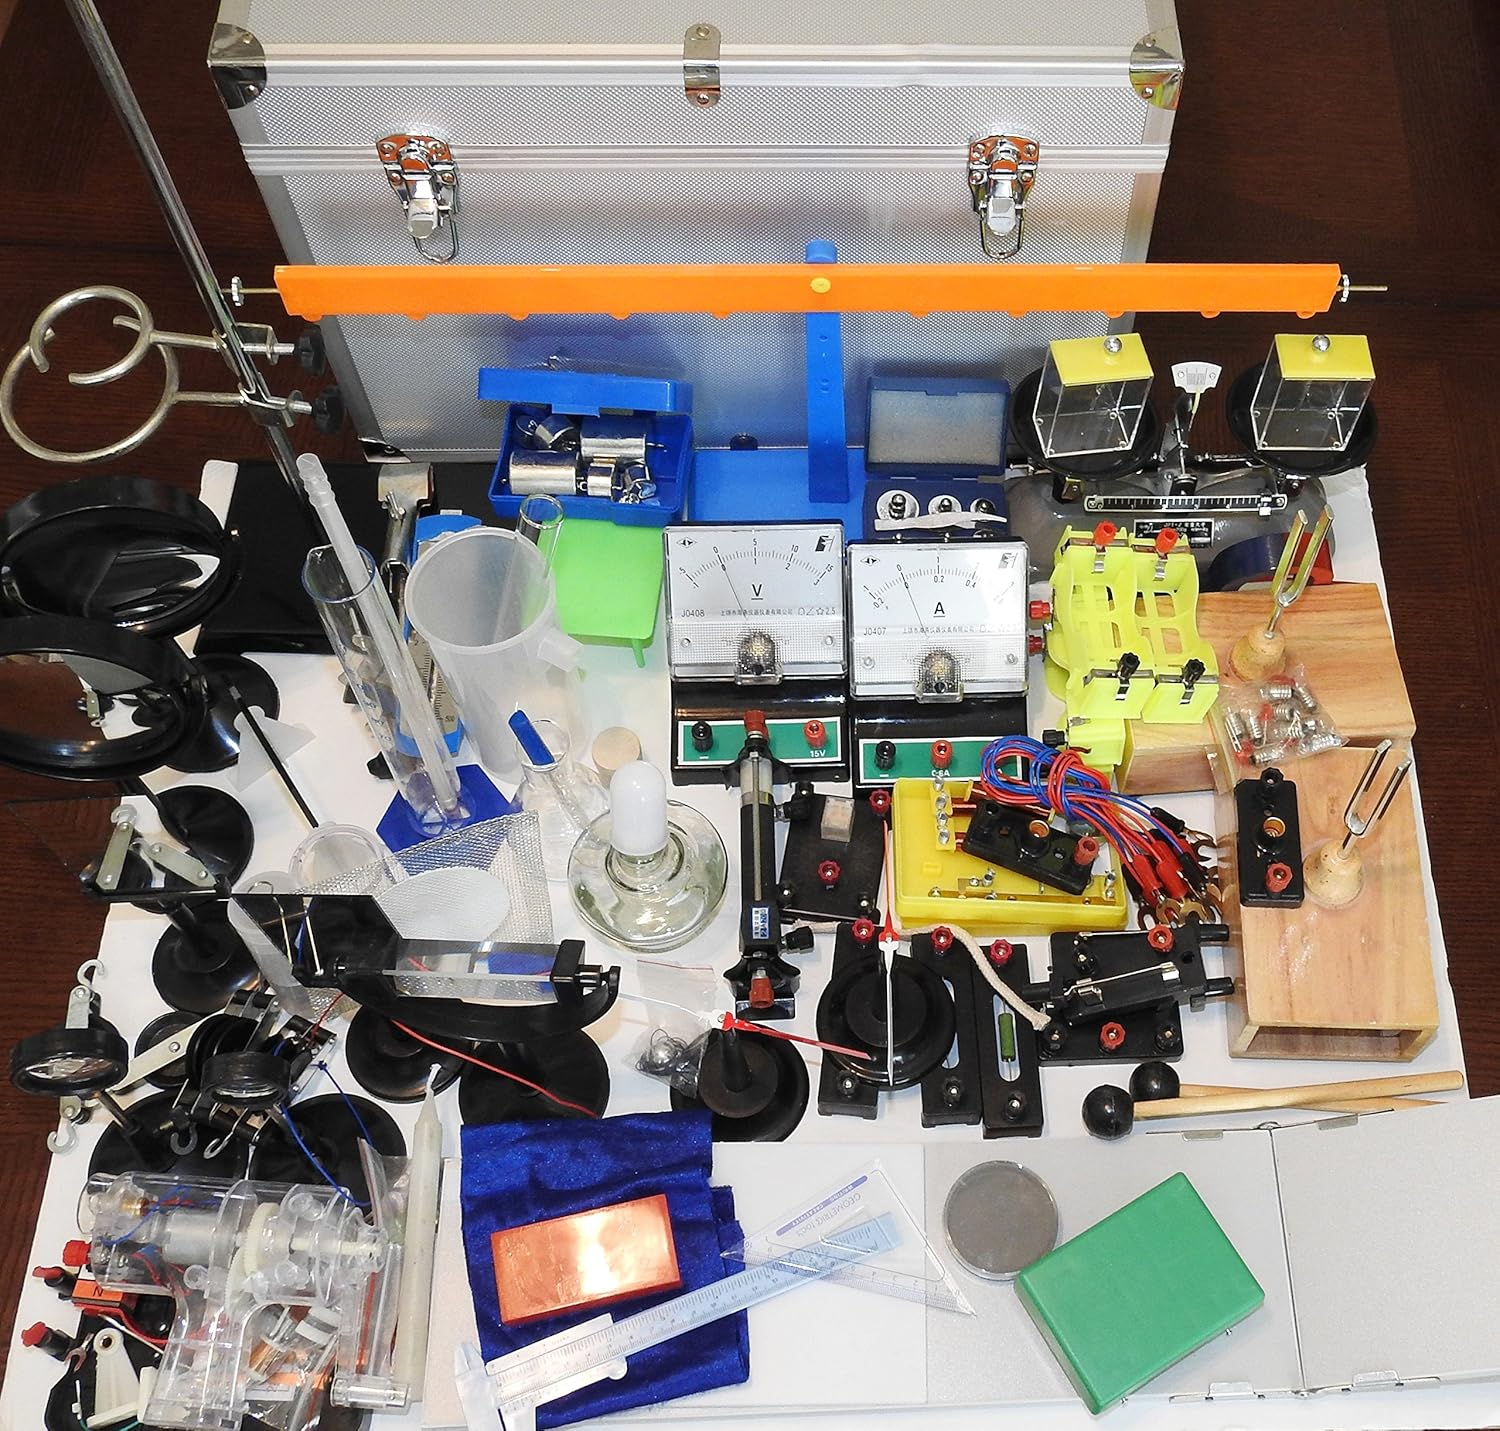
\includegraphics[width=0.3\textwidth]{imagenes/ejemplo_1.jpg}
  \caption{Diagrama del montaje experimental.}
  \label{fig:montaje}
\end{figure}

\subsection{Ejemplo con altura fija y posición \texttt{[h!]}}

\begin{figure}[h!]
  \centering
  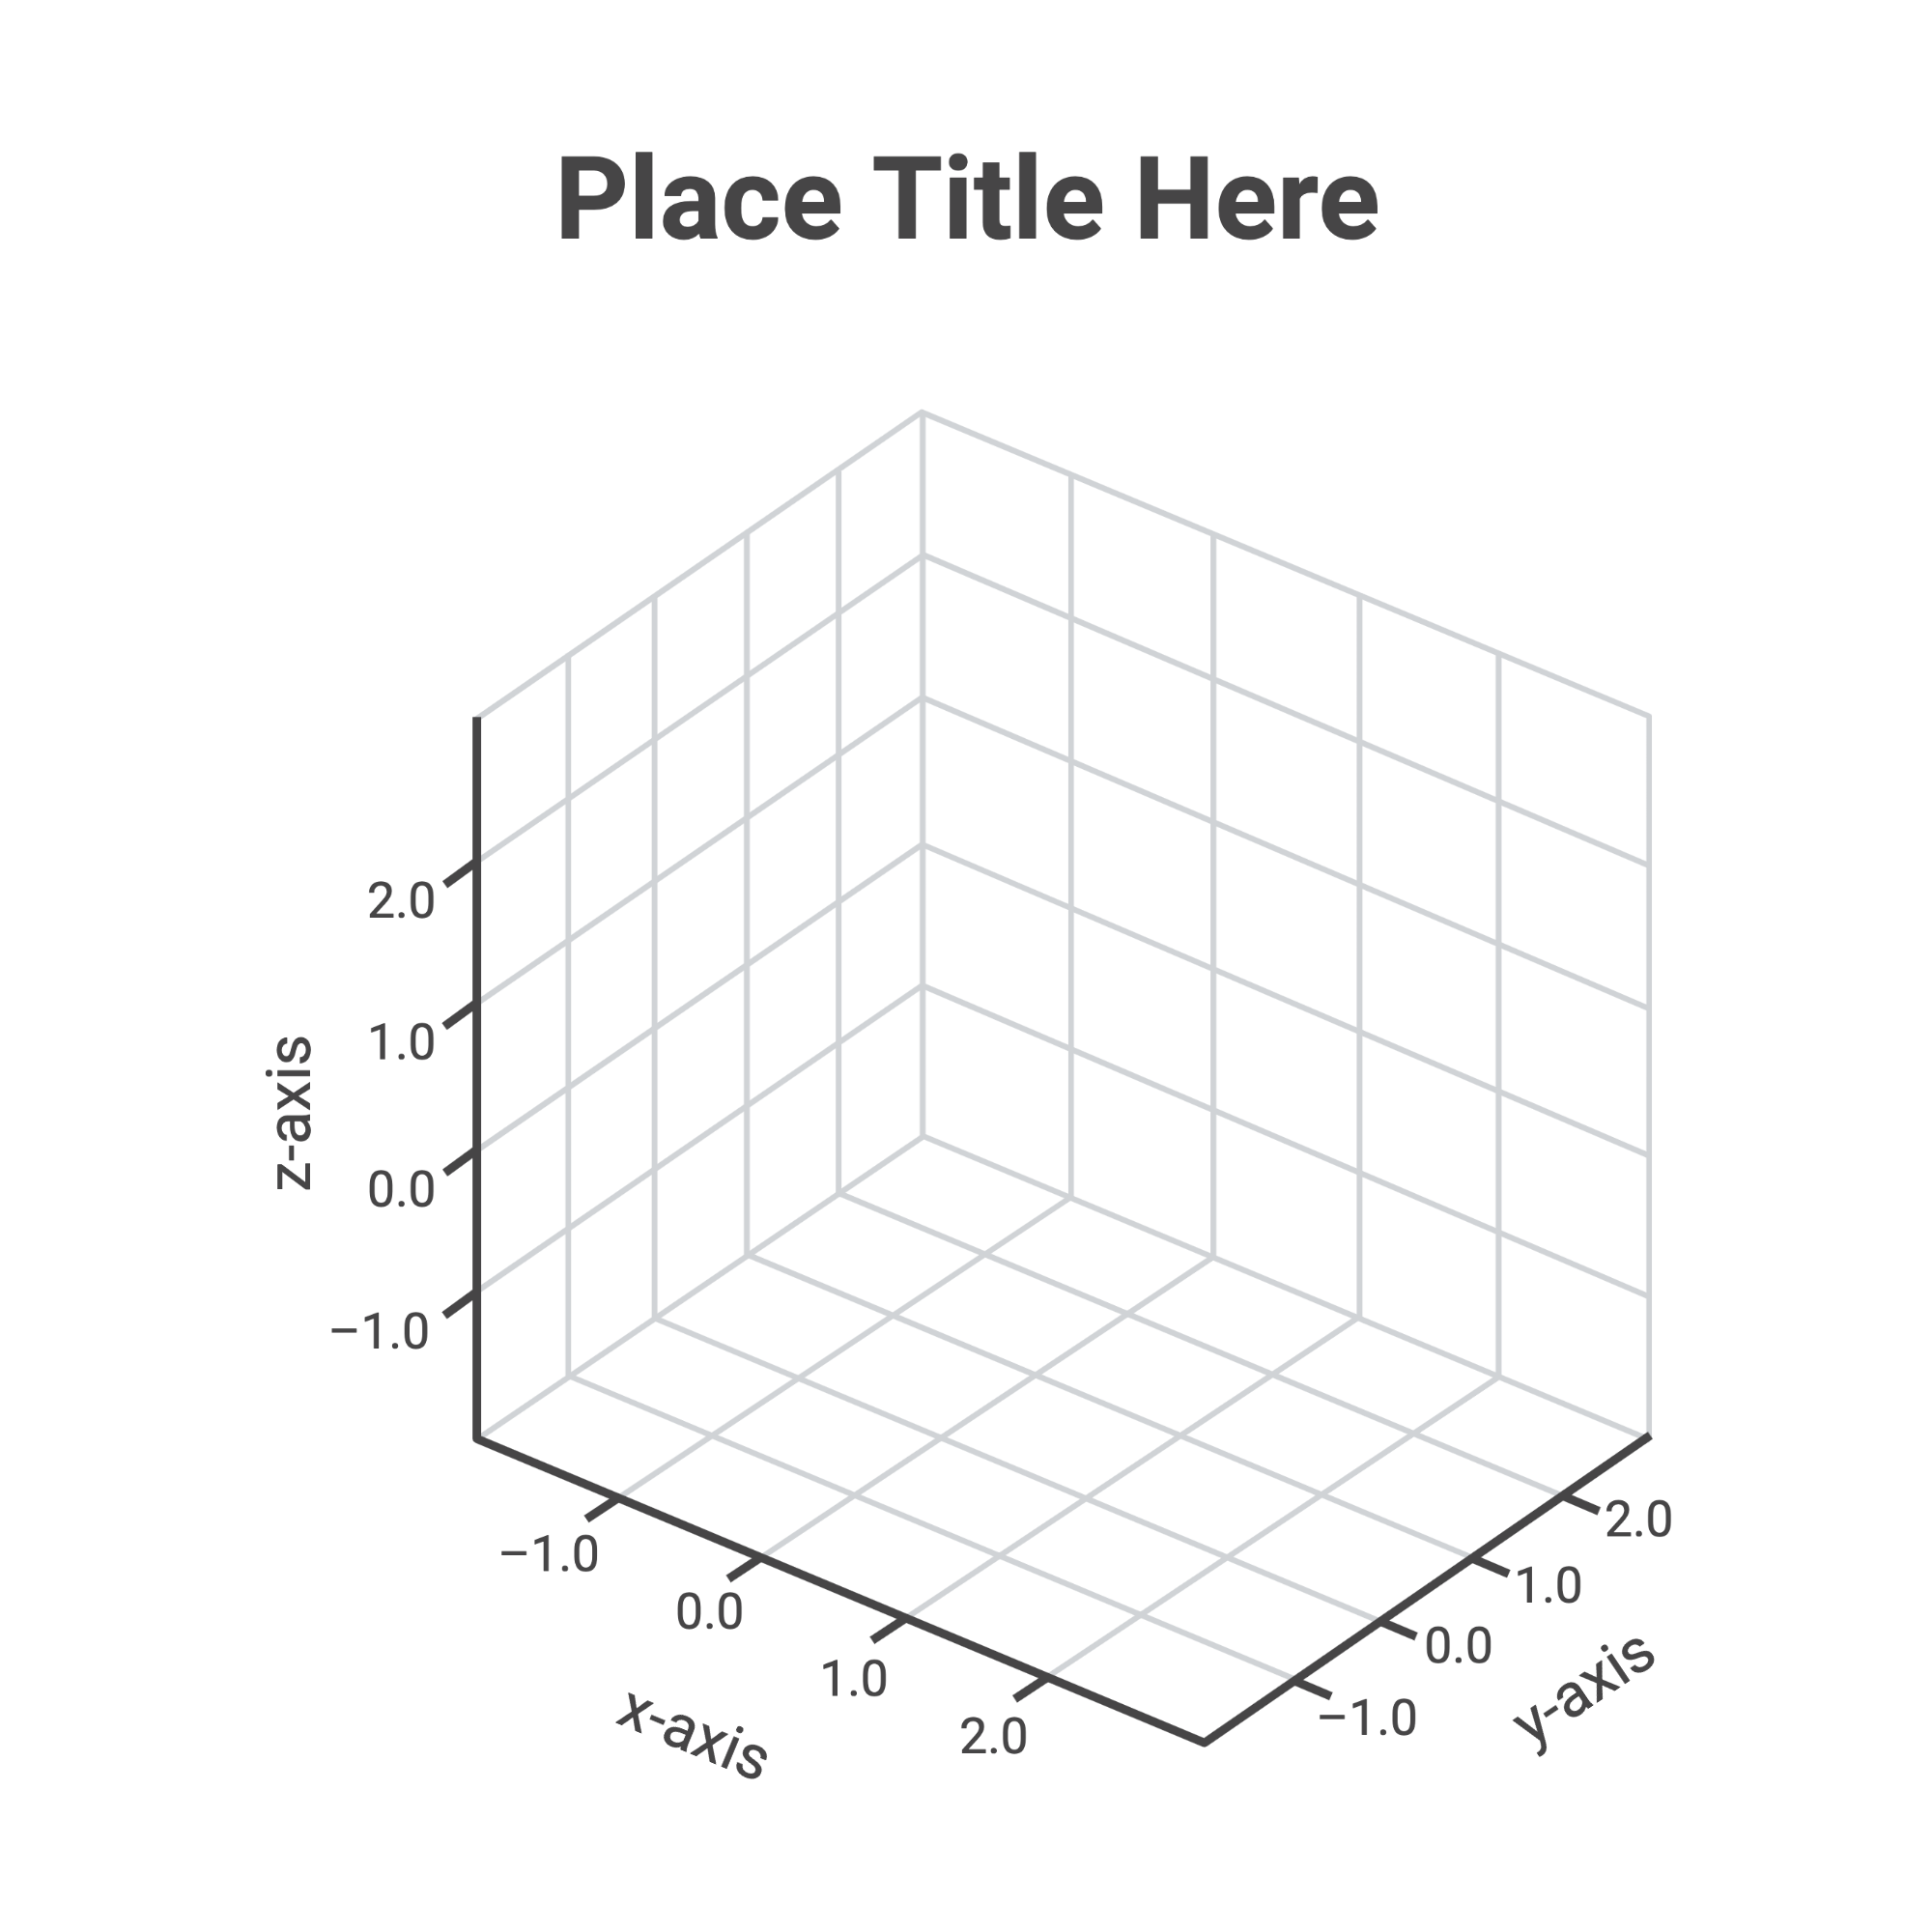
\includegraphics[height=4cm]{imagenes/ejemplo_grafica.png}
  \caption{Gráfica de calibración.}
  \label{fig:calibracion}
\end{figure}

\subsection{Referencia a una imagen}

Como se ve en la Figura~\ref{fig:montaje}, el montaje consiste en...

\newpage

\section{Tablas}

Las tablas se crean con el entorno \texttt{tabular} dentro de \texttt{table}.

\subsection{Tabla sin bordes}

\begin{table}[htbp]
  \centering
  \begin{tabular}{l c r}
    Masa (g) & Longitud (cm) & Período (s) \\
    50.0 & 20.0 & 0.89 \\
    100.0 & 20.0 & 0.90 \\
    150.0 & 20.0 & 0.91 \\
  \end{tabular}
  \caption{Datos brutos (sin bordes).}
  \label{tab:sin_bordes}
\end{table}

\subsection{Tabla con bordes completos (líneas verticales y horizontales)}

\begin{table}[htbp]
  \centering
  \begin{tabular}{|l|c|r|}
    \hline
    Masa (g) & Longitud (cm) & Período (s) \\
    \hline
    50.0 & 20.0 & 0.89 \\
    100.0 & 20.0 & 0.90 \\
    150.0 & 20.0 & 0.91 \\
    \hline
  \end{tabular}
  \caption{Datos con bordes completos.}
  \label{tab:bordes_completos}
\end{table}

\subsection{Tabla con bordes parciales (solo horizontales, estilo profesional con \texttt{booktabs})}

Primero carga el paquete \texttt{booktabs} en el preámbulo:
\verb|\usepackage{booktabs}|

\begin{table}[htbp]
  \centering
  \begin{tabular}{l c r}
    \toprule
    Masa (g) & Longitud (cm) & Período (s) \\
    \midrule
    50.0 & 20.0 & 0.89 \\
    100.0 & 20.0 & 0.90 \\
    150.0 & 20.0 & 0.91 \\
    \bottomrule
  \end{tabular}
  \caption{Tabla con reglas \texttt{booktabs} (recomendada).}
  \label{tab:booktabs}
\end{table}
\newpage
\subsection{Tabla con celdas combinadas}

\begin{table}[htbp]
  \centering
  \begin{tabular}{|c|c|c|}
    \hline
    \multicolumn{3}{|c|}{Mediciones de temperatura} \\
    \hline
    Tiempo (min) & Temp. (°C) & Error (±°C) \\
    \hline
    0 & 22.5 & 0.2 \\
    5 & 25.1 & 0.2 \\
    10 & 27.8 & 0.2 \\
    \hline
  \end{tabular}
  \caption{Uso de \texttt{\textbackslash multicolumn}.}
  \label{tab:multicol}
\end{table}

\subsection{Tabla que ocupa todo el ancho de la página (\texttt{tabularx})}

Carga el paquete: \verb|\usepackage{tabularx}|

\begin{table}[htbp]
  \centering
  \begin{tabularx}{\textwidth}{|X|X|X|}
    \hline
    Variable & Valor medido & Unidad \\
    \hline
    Resistencia & 47.2 & k$\Omega$ \\
    Capacitancia & 100 & $\mu$F \\
    Voltaje pico & 5.0 & V \\
    \hline
  \end{tabularx}
  \caption{Tabla ancha con columnas automáticas.}
  \label{tab:tabularx}
\end{table}

\subsection{Referencia a una tabla}

Los resultados se resumen en la Tabla~\ref{tab:booktabs}.  
Se recomienda usar el estilo \texttt{booktabs} para informes científicos.